\documentclass[../piano-di-progetto.tex]{subfiles}

\begin{document}

  \subsection{Progettazione della technology baseline}

  \subsubsection{Prospetto orario}
  Nel periodo di Progettazione della technology baseline, la distribuzione oraria è la seguente:
  \begin{table}[H]
    \centering
    \begin{tabular}{lccccccc}
      \rowcolor{lightgray}
      \textbf{Nominativo}        & \textbf{Re} & \textbf{Am}  & \textbf{An} & \textbf{Pt}  & \textbf{Pr}   & \textbf{Ve} & \textbf{Ore totali} \\
      Sofia Bononi              & -           & -           & -           & 7           & 9           & 11          & 27           \\
      Enrico Buratto            & 7           & -           & 6           & 5           & -           & 10          & 28           \\
      Ian Nicolas Di Menna      & -           & -           & 8           & 5           & 7           & 9           & 29           \\
      Alessandro Franchin       & -           & 9           & 5           & 6           &             & 9           & 29           \\
      Enrico Galdeman           & 7           & -           & -           & 5           & 6           & 10          & 28           \\
      Nicholas Miazzo           & -           & 9           & -           & 5           & 5           & 9           & 28           \\
      Marco Nardelotto          & -           & -           & 5           & 6           & 6           & 10          & 27           \\
      \textbf{Ore totali ruolo} & \textbf{14} & \textbf{18} & \textbf{24} & \textbf{39} & \textbf{33} & \textbf{68} & \textbf{196}
    \end{tabular}
    \caption{Distribuzione oraria del periodo di Progettazione della technology baseline}
  \end{table}


  Per facilitare la lettura della distribuzione oraria, i dati vengono rappresentati graficamente mediante il seguente istogramma:
  \begin{figure}[H]
    \centering
    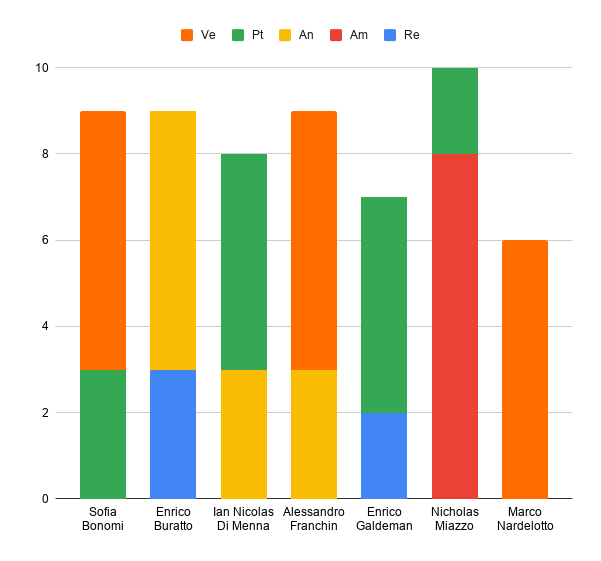
\includegraphics[width=12cm]{img/ore-progettazione.png}
    \caption{Istogramma della distribuzione oraria del periodo di Progettazione della technology baseline}
    \label{fig:ore-componente-progettazione}
  \end{figure}

  \subsubsection{Prospetto economico}
  In questo periodo, la suddivisione oraria e i costi per ruolo è la seguente:

  \begin{table}[H]
    \centering
    \begin{tabular}{lcc}
      \rowcolor{lightgray}
      \textbf{Ruolo}  & \textbf{Ore previste} & \textbf{Costo}  \\
      Responsabile    & 14           & € 420,00            \\
      Amministratore  & 18           & € 360,00            \\
      Analista        & 24           & € 600,00            \\
      Progettista     & 39           & € 858,00            \\
      Programmatore   & 33           & € 495,00            \\
      Verificatore    & 68           & € 1.020,00          \\
      \textbf{Totale} & \textbf{196} & \textbf{€ 3.753,00}
    \end{tabular}
    \caption{Prospetto economico del periodo di progettazione della technology baseline}
  \end{table}


  Per facilitare la lettura della suddivisione oraria per ruolo, i dati vengono rappresentati graficamente mediante il seguente areogramma:
  \begin{figure}[H]
    \centering
    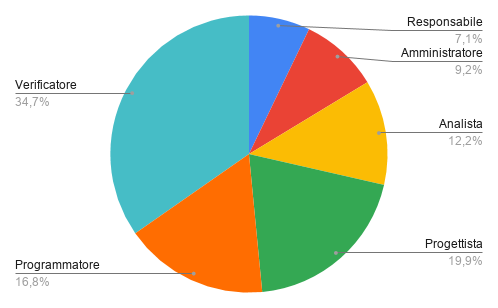
\includegraphics[width=12cm]{img/ruoli-progettazione.png}
    \caption{Areogramma della suddivisione dei ruoli del periodo di Progettazione della technology baseline}
    \label{fig:ore-ruolo-progettazione}
  \end{figure}

\end{document}
